\documentclass[journal]{IEEEtran}
\usepackage[utf8]{inputenc}
\usepackage{amsmath}
\usepackage{amsfonts}
\usepackage{amssymb}
\usepackage{graphicx}
\usepackage[left=2cm,right=2cm,top=2cm,bottom=2cm]{geometry}
\usepackage[export]{adjustbox}
\usepackage{subfigure,color,amsmath,amssymb,amsfonts}
\usepackage{url,graphicx,subfigure}

% Some handy Latin commands
\newcommand{\etal}{\textit{et al}.}
\newcommand{\ie}{\textit{i}.\textit{e}.,}
\newcommand{\eg}{\textit{e}.\textit{g}.}

\begin{document}
\title{Simulation of IEEE 802.11a PHY Layer}
\author{Alon S. Levin\thanks{The Cooper Union, Department of Electrical Engineering}\\Wireless Communications\\ECE-408 --- Spring 2020}
\maketitle

\begin{abstract}
The 1997 release of IEEE's 802.11 standard marked the advent of wireless local access networking (WLAN) usage. Since then, IEEE has released multiple amendments to its original protocol designation, the first of which --- 802.11a --- defined an OFDM-based air interface operating in the 5 GHz frequency band. The purpose of this report is to model the physical layer of this standard and compare empirical bit error rates (BER) across the different defined modulation schemes. The standard is broken down into individual block components, and a MATLAB simulation is presented.
\end{abstract}

\begin{IEEEkeywords}
IEEE 802.11a, OFDM, wireless communication networks
\end{IEEEkeywords}

%%%%%%%%%%%%%%%%%%% Introductions %%%%%%%%%%%%%%%%%%
\section{Introduction}\label{sec:intro}
Although the first wireless local access network (WLAN) was implemented in 1971 by Norman Abramson, wireless internet only became commercially viable with the development of IEEE's 802.11 series of protocols. Since its initial release in 1997, the protocols have seen numerous amendments, the first of which was released in 1998 under the title \emph{IEEE 802.11a}. This standard built upon its predecessor by defining an OFDM-based air interface that would operate on the 5 GHz frequency band, thereby reducing congestion on the 2.4 GHz band.

The 802.11a protocol was the first wireless standard to use OFDM techniques for packet transmission. The standard allows for a maximum data rate of 54 Mbps, with allowance for reduction to 48, 36, 24, 18, 12, 9, and 6 Mbps in cases of severe signal degradation by changing the modulation and coding rate used to relay the data. Although the higher-frequency of operation lends to a decreased effective overall range, this fact is made up for by the propagation advantages offered by OFDM, especially in multipath environments.

This report will break down the components of the 802.11a PHY layer, beginning with OFDM modulation and progressing backwards along the transmitter's components.

\section{Description of the Standard} \label{sec:standard_components}
The standard defines a total of eight data transmission schemes, characterized by their data rates and modulation schemes. This is shown in Fig.~\ref{fig:rate_params}, which presents the key rate-dependent parameters of this protocol.
\begin{figure}
    \centering
    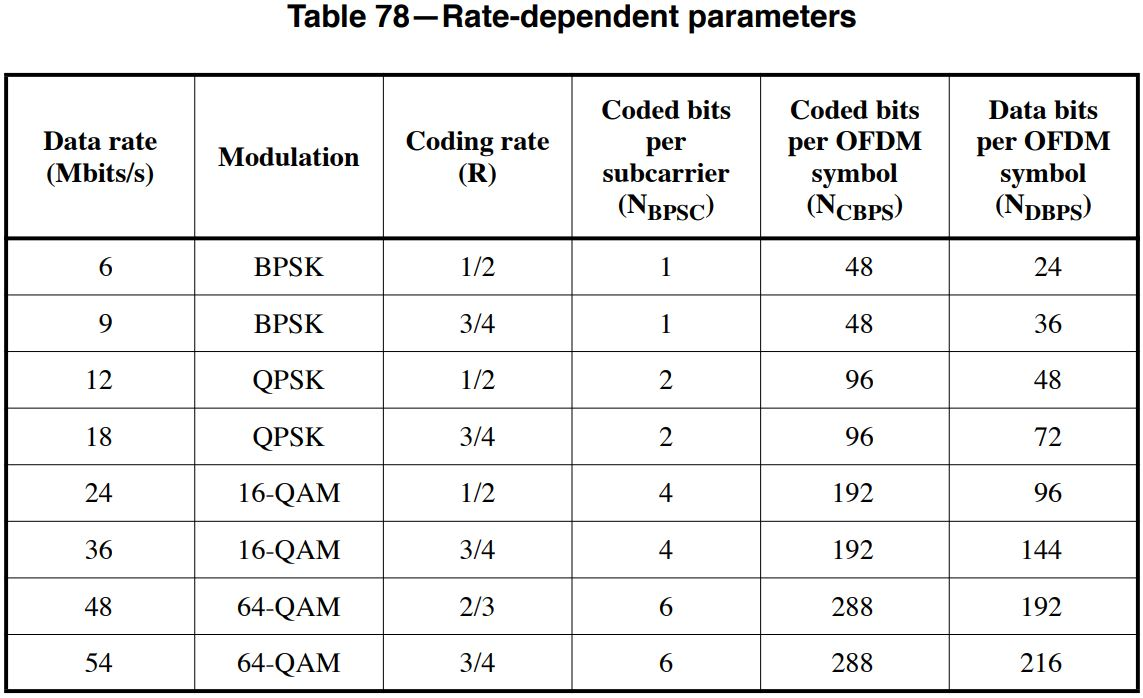
\includegraphics[width = 0.45\textwidth]{RateDepParams}
    \caption{Recreation of Table 78 --- Rate-Dependent Parameters}
    \label{fig:rate_params}
\end{figure}

In all eight modes of operation, timing parameters remain constant. These are represented in Fig~\ref{fig:time_params}.
\begin{figure}
    \centering
    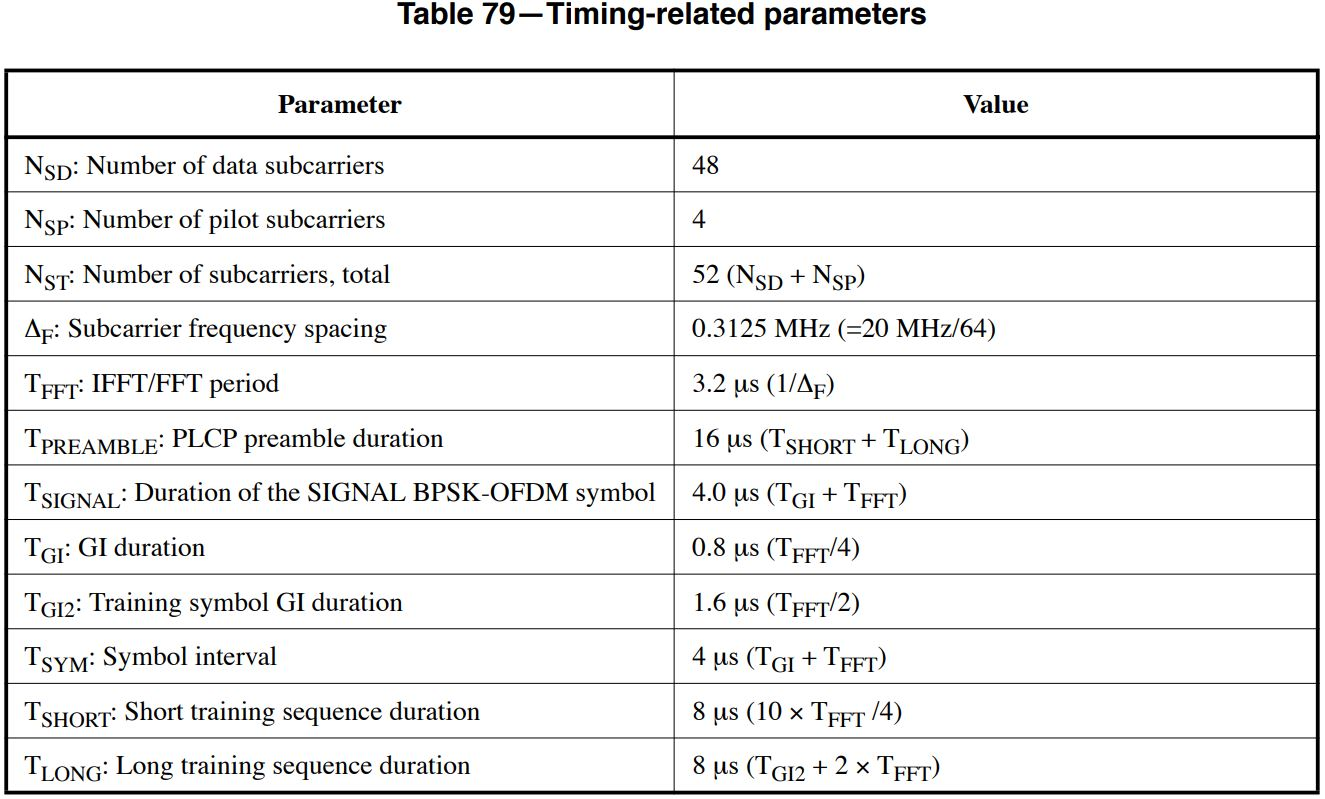
\includegraphics[width = 0.45\textwidth]{TimeDepParams}
    \caption{Recreation of Table 79 --- Timing-Related Parameters}
    \label{fig:time_params}
\end{figure}

Channels in the 5 GHz band are defined by their center frequencies, using the relation
\begin{equation}
\text{f}_\text{c} = 500 + 5 \times \text{n}_\text{ch},
\end{equation}
where $\text{n}_\text{ch} = 0,1,...,200$. However, due to regulation, not all channels are available for use; for the purpose of this project channel 36 was used in determining the center frequency.

\subsection{OFDM} \label{sec:OFDM}
OFDM, or \emph{Orthogonal Frequency-Division Multiplexing}, is a modulation scheme by which digital data is encoded onto multiple carrier frequencies within a certain frequency band, all spaced $\Delta_\text{F} = 1/\text{T}_\text{FFT}$ MHz apart. There is an additional condition that all subcarrier signals must be orthogonal to each other on the channel, thereby all but eliminating inter-carrier interference (ICI) and removing the need to include inter-carrier guard bands in the frequency domain (consequently allowing for a high spectral efficiency). An example of an OFDM spectrum across five subcarriers is presented in Fig~\ref{fig:OFDM}.
\begin{figure}
    \centering
    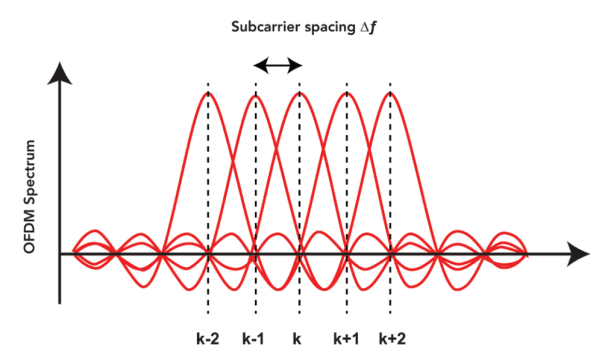
\includegraphics[width = 0.45\textwidth]{OFDM}
    \caption{Illustration of OFDM spectrum.}
    \label{fig:OFDM}
\end{figure}

This orthogonality principle lends to simple hardware translation as, fundamentally, one can use an inverse-forward pair of Fast Fourier Transform (FFT) blocks to facilitate this modulation on the transmitter and receiver, respectively. The 802.11 standard encodes forty-eight symbols at a time; combined with four pilot subcarriers, the frame is passed through a zero-padded IFFT (as shown in Fig.~\ref{fig:IFFT}).
\begin{figure}
    \centering
    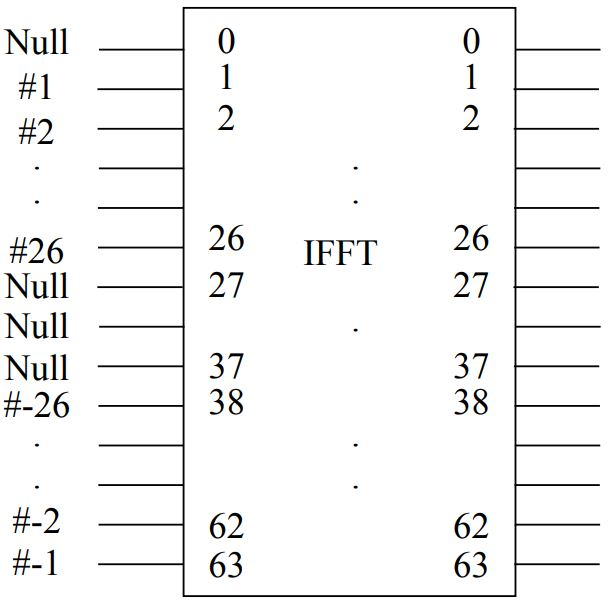
\includegraphics[width = 0.25\textwidth]{IFFT}
    \caption{Block diagram of symbol ordering on input to IFFT on the transmitter.}
    \label{fig:IFFT}
\end{figure}

Once in the time-domain, a cyclic prefix is prepended to the frame, consisting of the last sixteen time-domain samples out of the outputted sixty-four. This is easily apparent as, per Fig.~\ref{fig:time_params}, the required guard time $\text{T}_\text{GI}$ (which determines the time-frame that the cyclic prefix occupies) is a quarter of the IFFT/FFT period $\text{T}_\text{FFT}$. Therefore, the entire transmitted frame consists of a total of eighty time-domain samples (see Fig.~\ref{fig:Frame}).
\begin{figure}
    \centering
    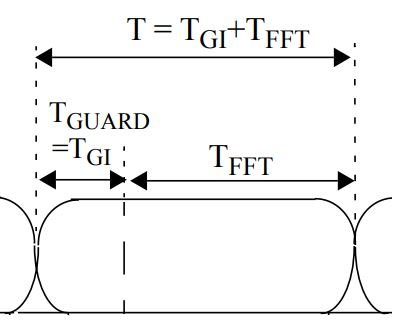
\includegraphics[width = 0.45\textwidth]{Frame}
    \caption{A single time-domain transmission frame, with guard time $\text{T}_\text{GI}$ and useful symbol time $\text{T}_\text{FFT}$ labeled.}
    \label{fig:Frame}
\end{figure}

At this stage, the signal is heterodyned for RF transmission across the channel, where it is received by the receiver, heterodyned back down to baseband, and OFDM demodulation takes place.

\subsection{Baseband Modulation} \label{sec:Modulation}
The set of forty-eight symbols transmitted to the IFFT block for OFDM modulation must first be obtained from the raw binary data.  The 802.11a standard defines four specific modulation schemes for this purpose:
\begin{itemize}
\item Binary Phase Shift-Keying (BPSK)
\item Quadrature Phase-Shift Keying (QPSK)
\item 16-Quadrature Amplitude Modulation (16-QAM)
\item 64-Quadrature Amplitude Modulation (64-QAM)
\end{itemize}

The constellation diagrams of these four schemes are shown in Fig.~\ref{fig:Constellations}. Note the use of Gray code in symbol assignment. Finally, a normalization factor $\text{K}_\text{mod}$ dependent on the base modulation mode is multiplied against the modulated symbols, as a means of achieving the same average power across all mappings. On the demodulator end, the received symbols are initially divided by the normalization factor to allow for proper demodulation.
\begin{figure}
    \centering
    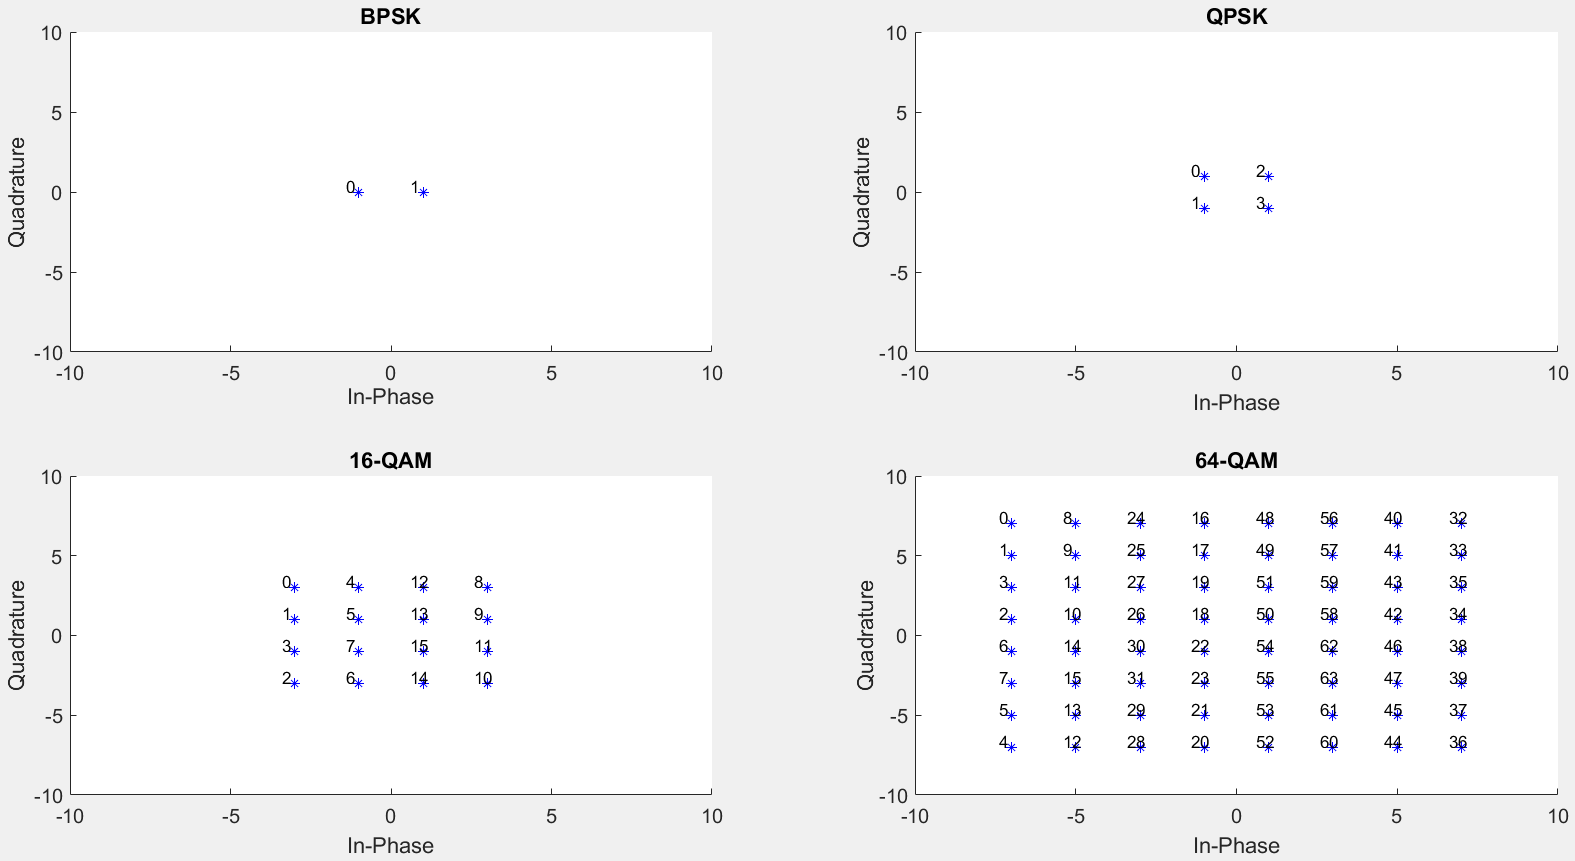
\includegraphics[width = 0.45\textwidth]{Modulation}
    \caption{Constellation diagrams of the modulation schemes used in IEEE 802.11a.}
    \label{fig:Constellations}
\end{figure}

\subsection{Error Correction \& Interleaving} \label{sec:ErrorCorrect}
The 802.11a protocol utilizes two main methods for error-correction: convolutional coding and data interleaving. 

The convolutional encoder operates at one of three possible data rates: $\frac{1}{2}$, $\frac{3}{4}$, or $\frac{2}{3}$. All three  utilize the same trellis for data-generation, based on the industry-standard generator polynomials
\begin{eqnarray}
\nonumber g_0 = 133_8 \\
\nonumber g_1 = 171_8
\end{eqnarray}
that form the $k=7$ convolutional encoder shown in Fig.~\ref{fig:trellis}. In its original form, this encoder is a purely $\frac{1}{2}$ rate encoder; in order to achieve the higher data rates, the standard calls for the employment of \emph{puncturing} --- the process of omitting some encoded bits in the transmitter and replacing them with a dummy ``zero" bit on the receiver side. In all three cases, a Viterbi decoder is used to recapture the original data bits.

In addition to convolutional coding, the standard requires the encoded message to be interleaved in order to mitigate burst errors. The standard requires a two-step block interleaving process, defined by two permutations: given an encoded signal of length $\text{N}_\text{CBPS}$ bits, the new index $j$ of bit $k$ is at
\begin{eqnarray}
\nonumber i = \frac{\text{N}_\text{CBPS}}{16}(k~\text{mod}~16) + \nonumber \text{floor}(\frac{k}{16}) \\
\nonumber k = 0,1,...,\text{N}_\text{CBPS}-1 \\
\nonumber j = s \times \text{floor}(\frac{i}{s}) + (i + \text{N}_\text{CBPS} - \text{floor}(\frac{16i}{\text{N}_\text{CBPS}}))~\text{mod}~s \\
\nonumber i = 0,1,...,\text{N}_\text{CBPS}-1, s = \text{max}(\frac{\text{N}_\text{CBPS}}{2}, 1)
\end{eqnarray}
Likewise, at the receiver, a deinterleaver block is also defined by two permutations (not listed here).

In addition, some implementations employ a matrix interleaver before the general block interleaver. In this simulation, the bits are inserted into a 16-column matrix, and reshaping back into a vector; this ensures that adjacent coded bits are mapped onto nonadjacent subcarriers, in the case of significant signal degradation on a single subfrequency.

\begin{figure}
    \centering
    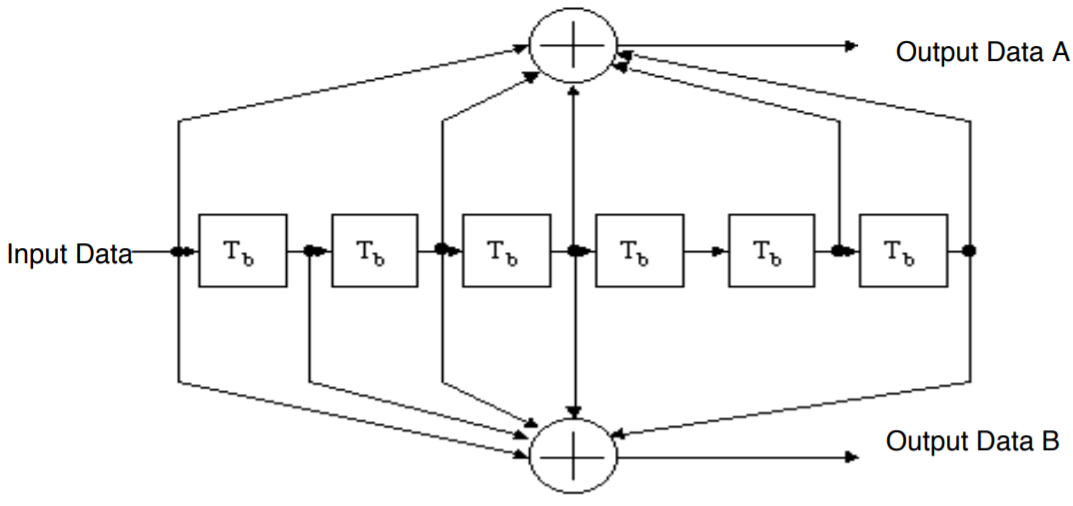
\includegraphics[width = 0.45\textwidth]{Trellis}
    \caption{Convolutional encoder.}
    \label{fig:trellis}
\end{figure}


\section{Channel Model \& Simulation} \label{sec:simulation}
\subsection{Channel Model}
Once fully formed, the signal was transmitted through a wireless channel before being picked up by the receiver. For the purposes of this simulation, a simple additive white Gaussian noise (AWGN) channel was used over a varying range of SNR levels, from -10 dB to 9 dB. 

\subsection{Simulation}
Twenty packets of information were transmitted at each of the eight data rates over all twenty SNR levels, for a total of $20\times8\times20 = 3,200$ packets transmitted. These packets were all transmitted sequentially over Channel 36 of the 5 GHz band. The average bit error rate (BER) per data rate per SNR level was calculated, and the results are shown in Fig.~\ref{fig:results_linear}-\ref{fig:results_log}.

\begin{figure}
    \centering
    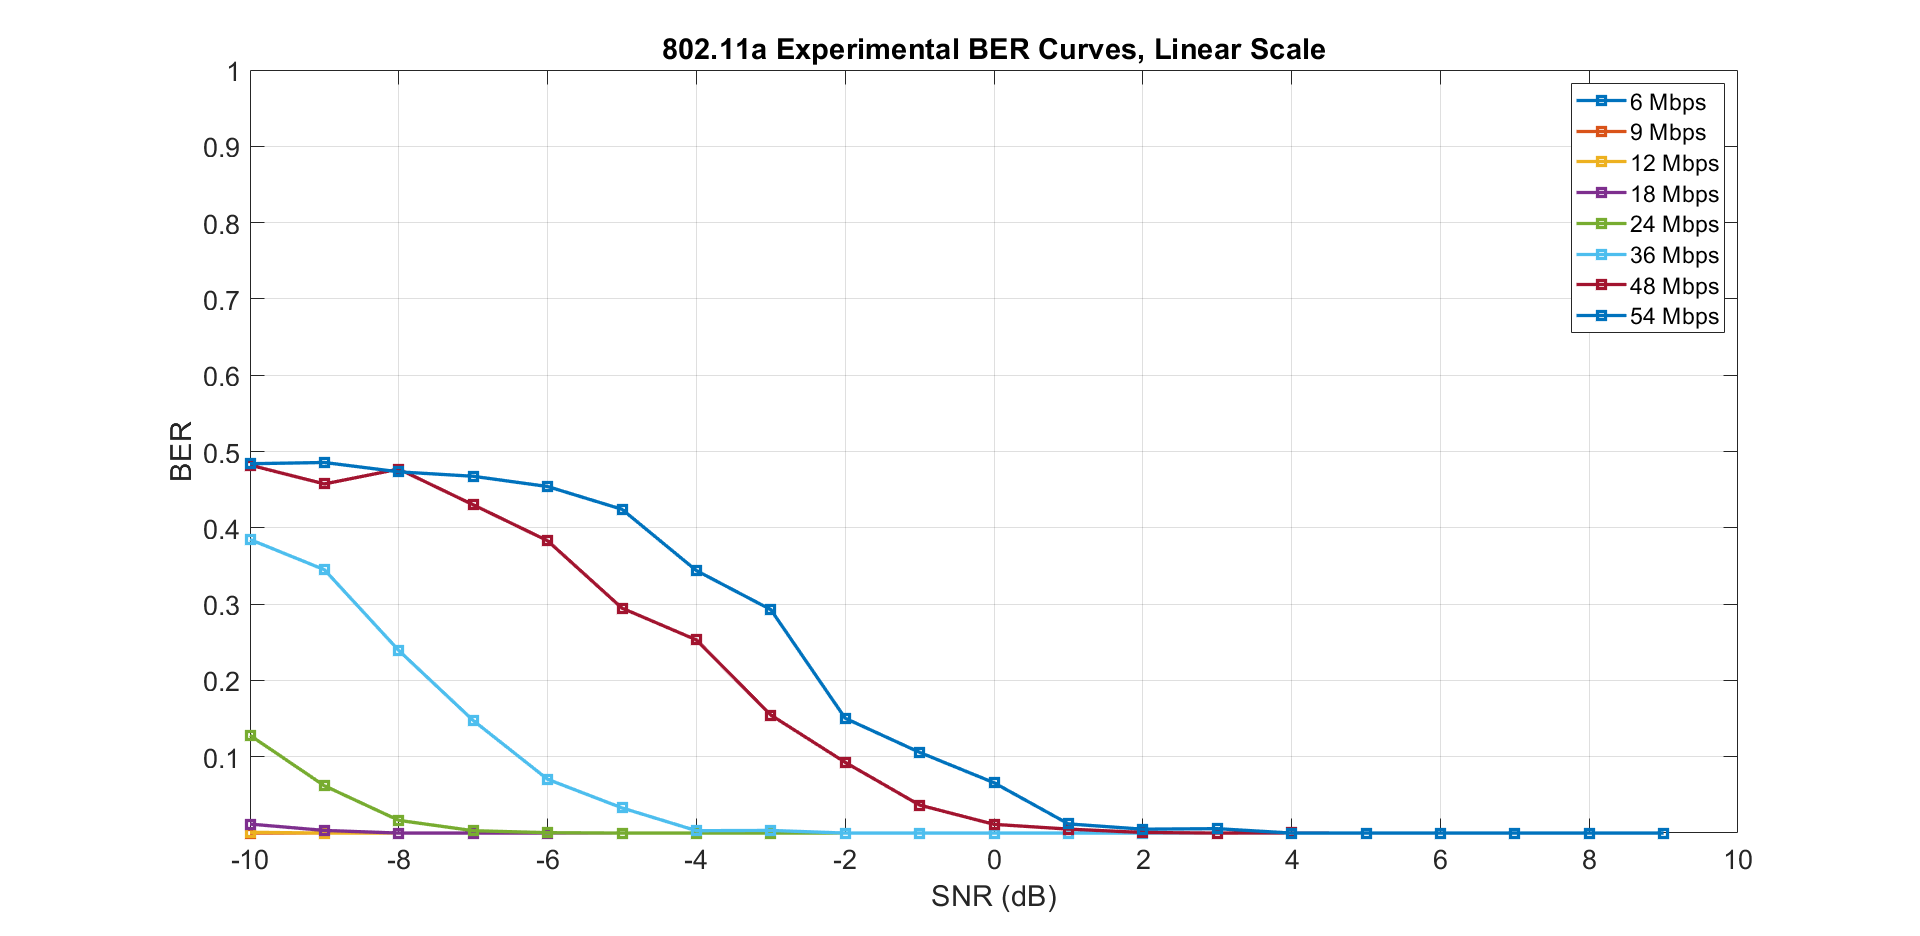
\includegraphics[width = 0.45\textwidth]{LinearScale}
    \caption{Empirical bit error rates versus SNR, linear scale.}
    \label{fig:results_linear}
\end{figure}
\begin{figure}
    \centering
    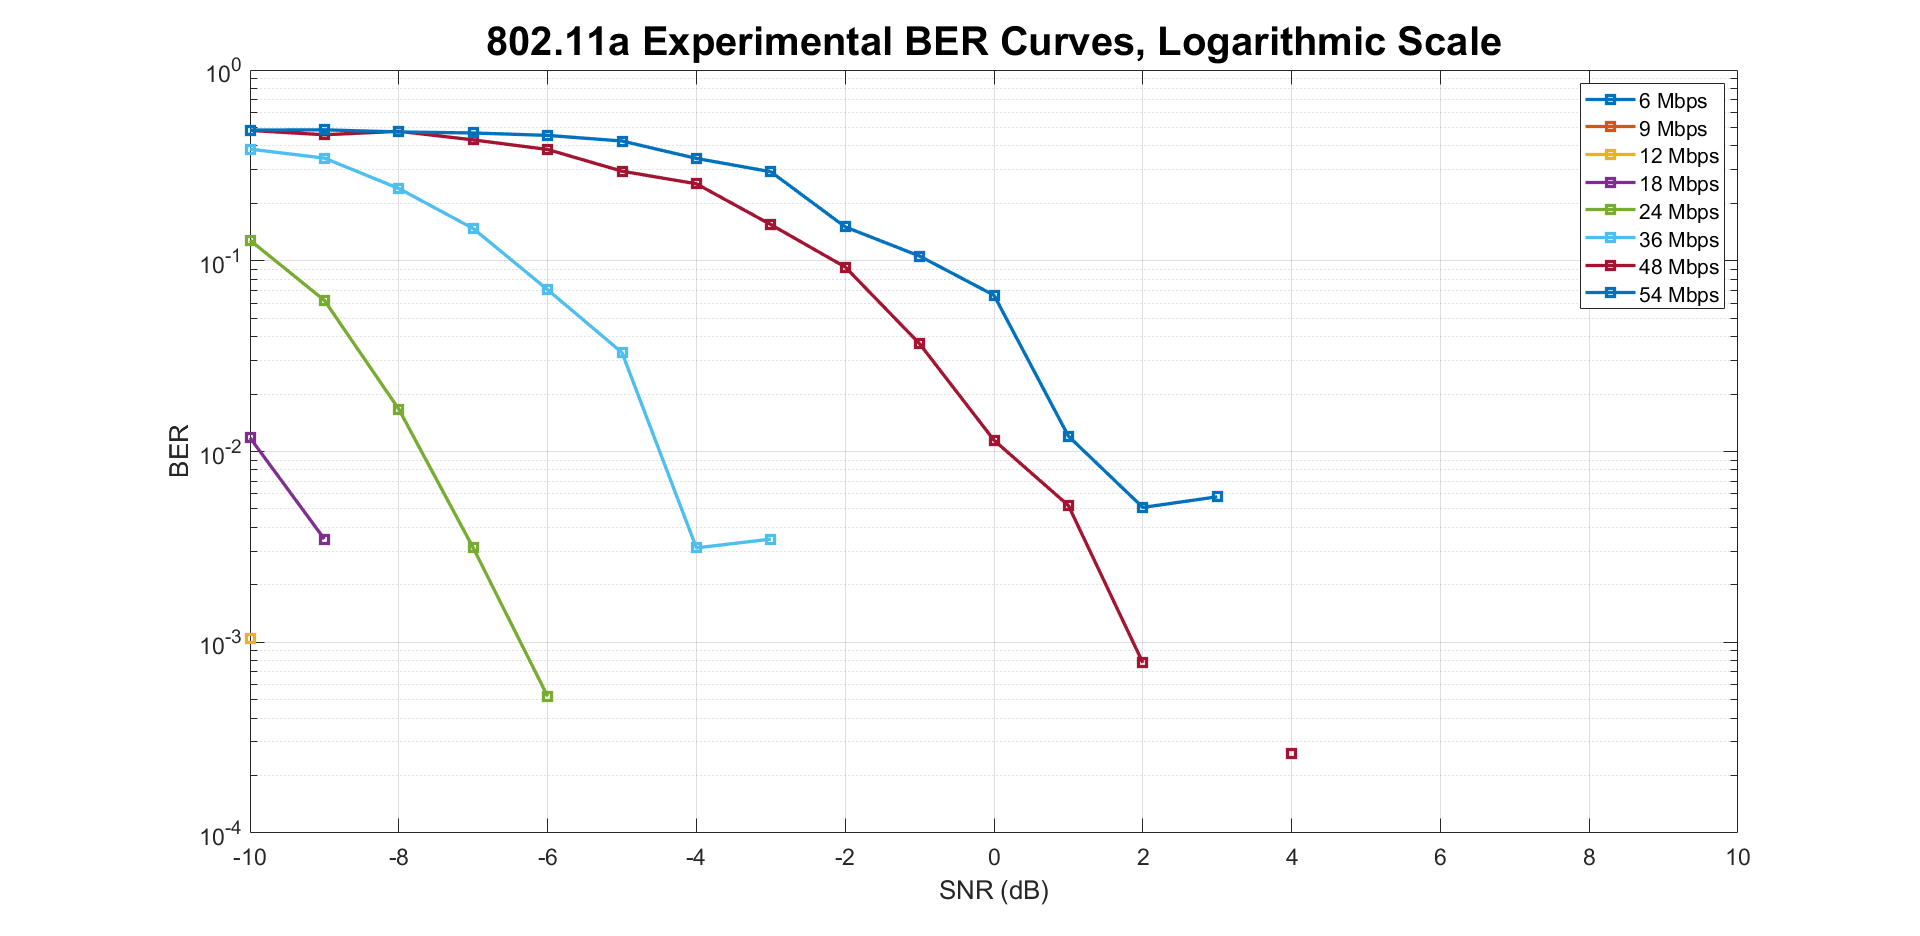
\includegraphics[width = 0.45\textwidth]{LogScale}
    \caption{Empirical bit error rates versus SNR, logarithmic scale.}
    \label{fig:results_log}
\end{figure}

\section{Results \& Conclusion}
The results clearly show very good behavior, even in the face of extremely poor channel conditions. Of the eight modulation schemes described in the standard, the two slowest rates showed the best performance, to the point of consistently showing a zero bit error rate across all channels attempted. At zero SNR, all eight schemes performed at a bit error rate of less than $10\%$, and at positive SNRs the bit error was effectively negligible. 

In hardware implementations, the implication here is that Wi-Fi systems operating on 802.11a can adapt their data transmission rates based upon channel conditions; if the bit error on the receiver side is too high, a lower data rate and smaller constellation can be changed to on the transmitter side. This strong performance and adaptability easily explain the widespread adoption of the standard in both residential and corporate settings.

Extensions of this project would include increasing the degradation in the channel, such as by accounting for quantization errors due to D\/A and A\/D conversion, simulating multi-path propagation, and considering the Doppler effects due to a mobile transmitter or receiver.


%%%%%%%%%%%%%%%%%%% Bibliography %%%%%%%%%%%%%%%%%%%
\bibliographystyle{unsrt}	
%% To reload citations:
%% F6 --> F11 --> F6 --> F6 --> F7
\bibliography{Bibliography} %filename (no .bib)

\end{document}